% =====================================================
% Advanced Programming 2025 - Project Report
% HEC Lausanne / UNIL
% =====================================================

\documentclass[11pt,a4paper]{article}

% ================== Encoding / Language ==================
\usepackage[utf8]{inputenc}
\usepackage[T1]{fontenc}
\usepackage[english]{babel}

% ================== Typography ==================
\usepackage{microtype} % better spacing/kerning (subtle but professional)

% ================== Math ==================
\usepackage{amsmath,amssymb,amsthm}

% ================== Figures / Tables ==================
\usepackage{graphicx}
\usepackage{float}
\usepackage{caption}
\usepackage{subcaption}
\usepackage{booktabs}   % professional tables
\usepackage{siunitx}    % aligned numbers in tables (optional but useful)
\sisetup{detect-all}

% ================== Colors / Code ==================
\usepackage{xcolor}
\usepackage{listings}

\definecolor{codegreen}{rgb}{0,0.55,0}
\definecolor{codegray}{rgb}{0.45,0.45,0.45}
\definecolor{codepurple}{rgb}{0.58,0,0.82}
\definecolor{backcolour}{rgb}{0.96,0.96,0.94}

\lstdefinestyle{pythonstyle}{
    backgroundcolor=\color{backcolour},
    commentstyle=\color{codegreen},
    keywordstyle=\color{magenta},
    numberstyle=\tiny\color{codegray},
    stringstyle=\color{codepurple},
    basicstyle=\ttfamily\footnotesize,
    breaklines=true,
    numbers=left,
    numbersep=6pt,
    showstringspaces=false,
    tabsize=2,
    language=Python,
    frame=single,
    framerule=0.2pt,
    rulecolor=\color{codegray}
}
\lstset{style=pythonstyle}

% ================== Page Layout ==================
\usepackage[margin=1in]{geometry}
\usepackage{fancyhdr}

% ================== Links / References ==================
\usepackage{csquotes} % recommended with biblatex
\usepackage{hyperref}
\hypersetup{
    colorlinks=true,
    linkcolor=blue,
    citecolor=blue,
    urlcolor=blue,
    pdftitle={An Early Warning System for Financial Crises},
    pdfauthor={Andrea Perani}
}
\usepackage[nameinlink,noabbrev]{cleveref} % nicer refs: "Figure 1", "Table 2"

% ================== Bibliography ==================
\usepackage[backend=biber,style=authoryear,maxcitenames=2]{biblatex}
\addbibresource{references.bib}

% ================== Header / Footer ==================
\pagestyle{fancy}
\fancyhf{}
\lhead{Project Report}
\rhead{Advanced Programming 2025}
\rfoot{Page \thepage}

% ================== Title ==================
\title{%
    \Large \textbf{Advanced Programming 2025} \\
    \vspace{0.4cm}
    \LARGE \textbf{An Early Warning System for Financial Crises} \\
    \vspace{0.2cm}
    \large Final Project Report
}

\author{
    Andrea Perani \\
    \texttt{andrea.perani@unil.ch}
}

\date{December 2025}

\begin{document}

\maketitle
\thispagestyle{empty}

% ================== Abstract ==================
% (We will rewrite this later once the Results section is finalized.)
\begin{abstract}
\noindent
This project develops a data-driven Early Warning System (EWS) for financial crises using weekly macro-financial indicators and modern machine learning techniques. The objective is to assess whether publicly available financial variables can provide timely and interpretable signals of increased systemic financial stress within a short forecasting horizon.

The analysis combines credit spreads, market volatility, yield-curve information, and dollar strength to predict the near-term exceedance of the St.\ Louis Financial Stress Index beyond a critical threshold. Early warning detection is formulated as a probabilistic binary classification problem and evaluated under a strictly time-consistent framework based on expanding-window cross-validation and a calendar-based hold-out test split. Model performance is assessed using metrics suited to rare-event prediction, including ROC-AUC and Average Precision.

Empirical results show that well-regularized linear models achieve strong and stable out-of-sample performance, outperforming more complex non-linear alternatives in this setting. Probability calibration further improves the reliability of predicted risk scores, enhancing their interpretability for monitoring purposes. Explainability analysis based on SHAP values indicates that credit spreads and market volatility are the primary drivers of predicted systemic risk, consistent with economic intuition and the literature on financial stability.

In general, the project delivers a transparent, reproducible, and interpretable early warning framework that bridges traditional financial risk monitoring with modern machine learning practice, while highlighting the trade-offs between model complexity, robustness, and practical applicability.
\end{abstract}

\vspace{0.4cm}
\noindent\textbf{Keywords:} early warning system, financial stress, time series, imbalanced classification, SHAP, calibration

\newpage
\tableofcontents
\newpage

% ================== Introduction ==================
\section{Introduction}
\label{sec:introduction}

Systemic financial crises are among the most disruptive events in modern economies, with severe consequences for financial markets, institutions, and real economic activity. Episodes such as the Global Financial Crisis of 2008 or the market turmoil during the COVID-19 pandemic illustrate how financial stress can accumulate gradually and then escalate rapidly, propagating across asset classes and amplifying economic downturns. Anticipating such developments before they fully materialize remains a central challenge for policymakers, regulators, and market participants.

Early Warning Systems (EWS) aim to address this challenge by identifying signals of increasing financial vulnerability before crisis episodes. Rather than producing deterministic predictions, effective early warning frameworks provide probabilistic assessments of future risk, allowing decision-makers to balance the costs of false alarms against the potentially severe consequences of missed crises. However, in practice, building reliable early warning signals is particularly difficult. Systemic stress events are rare, macro-financial indicators exhibit strong temporal dependence, and relationships between predictors and financial instability are often non-linear and unstable over time.

Traditional early warning approaches typically rely on econometric models or threshold-based rules applied to individual indicators such as credit growth, yield-curve inversions, or market volatility. Although transparent and interpretable, these methods may not capture complex interactions between indicators or adapt to changing financial regimes. Recent advances in machine learning offer new opportunities to enhance early warning systems by exploiting non-linear patterns and interactions in macro-financial data. At the same time, their application raises important methodological concerns, particularly regarding time-series validation, class imbalance, and model interpretability.

Against this background, this project investigates the feasibility of a data-driven Early Warning System based on weekly macro-financial indicators. The analysis focuses on short-horizon prediction and emphasizes probabilistic risk estimation under a strictly time-consistent and reproducible evaluation framework. The central research question of the project is the following:

\begin{quote}
\emph{Can weekly macro-financial indicators be used to estimate, in a probabilistic and interpretable manner, the likelihood of a near-term increase in systemic financial stress, under a strictly time-consistent evaluation framework?}
\end{quote}

To address this question, the project formulates early warning detection as a supervised binary classification problem and evaluates multiple machine learning models with varying degrees of complexity. Particular emphasis is placed on appropriate validation strategies for time-series data, evaluation metrics suited to rare-event prediction, and explainability tools that link model outputs to economically meaningful indicators.

% ================== Research Question & Literature ==================
\section{Research Question \& Literature}
\label{sec:literature}

\subsection{Research Question in Context}
\label{subsec:rq_context}

The research question introduced in the previous section is situated within the broad literature on Early Warning Systems for financial crises. The focus on probabilistic prediction of near-term increases in systemic financial stress reflects a shift away from deterministic crisis dating to risk-based monitoring frameworks. This perspective emphasizes timely detection of rising vulnerabilities rather than precise forecasting of crisis onset.

By framing early warning as a supervised classification problem with a short forecasting horizon, the analysis aligns with approaches that prioritize operational relevance and real-time applicability. The emphasis on weekly macro-financial indicators further reflects an interest in capturing rapidly evolving market conditions, while the requirement of strict time consistency addresses a key methodological concern in crisis prediction studies.

\subsection{Related Literature}
\label{subsec:related_literature}

Early contributions to financial crisis prediction are based on indicator-based and econometric approaches designed to identify warning signals from macroeconomic and financial variables. Kaminsky, Lizondo, and Reinhart~\cite{kaminsky1998} propose a signal extraction framework in which individual indicators issue warnings when exceeding predefined thresholds. Although transparent and intuitive, these methods often suffer from high false-alarm rates and limited ability to capture interactions between indicators.

Subsequent research emphasizes the role of credit conditions in the accumulation of systemic risk. Borio and Lowe~\cite{borio2002} show that measures of credit expansion and asset price imbalances provide valuable early warning information, particularly when evaluated jointly. These findings motivate the inclusion of credit spreads and yield-curve indicators in many early warning frameworks.

More recent studies apply machine learning techniques to overcome the limitations of linear and threshold-based models. Barboza, Kimura, and Altman~\cite{barboza2017} demonstrate that classification algorithms such as random forests and gradient enhancement can improve predictive performance by capturing non-linear relationships and complex interactions among macro-financial variables. At the same time, they stress the importance of appropriate validation strategies and evaluation metrics in rare-event settings.

In parallel, a related strand of literature focuses on constructing aggregate measures of financial distress. Boyarchenko, Kovner, and Shachar~\cite{boyarchenko2025} develop a Corporate Bond Market Distress Index based on corporate bond market data, highlighting the informational content of credit spreads for monitoring systemic risk and forecasting future economic activity.

\subsection{Positioning of This Study}
\label{subsec:positioning}

This project contributes to the literature by combining macro-financial indicators with machine learning techniques in a framework that explicitly prioritizes time-series consistency, interpretability, and reproducibility. Unlike traditional indicators-based approaches, the proposed system integrates multiple sources of financial information to produce probabilistic early warning signals rather than binary alarms.

Relative to previous machine learning applications, the main contribution lies in the design of a rigorous evaluation framework based on time-series–aware cross-validation and a strictly held-out test set. Furthermore, the integration of SHAP-based explainability links model predictions to economically meaningful drivers of systemic stress, addressing a common criticism of black-box approaches in financial applications.

By focusing on weekly data and a short forecasting horizon, the analysis complements studies that emphasize medium-term vulnerabilities and demonstrates how higher-frequency macro-financial indicators can be leveraged for timely and interpretable early warning.

% ================== Methodology ==================
\section{Methodology}
\label{sec:methodology}

\subsection{Data}
\label{subsec:data}

The Early Warning System is built on a set of weekly macro-financial indicators designed to capture multiple dimensions of systemic financial stress. All data used in the analysis are publicly available and are automatically retrieved through the project pipeline to ensure full reproducibility.

The dataset combines indicators obtained from two primary sources. Credit market and financial stress variables are sourced from the Federal Reserve Economic Data (FRED) database, while market-based indicators reflecting investor sentiment and global risk conditions are retrieved from Yahoo Finance.

Specifically, the following variables are included. Credit conditions are captured by the investment-grade and high-yield corporate bond option-adjusted spreads (IG\_OAS and HY\_OAS). Market uncertainty is proxied by the CBOE Volatility Index (VIX). The slope of the U.S.\ yield curve is measured as the difference between the 10-year and 2-year Treasury yields (T10Y2Y), reflecting expectations about future economic activity and monetary policy. Finally, global funding and risk-off dynamics are captured by the U.S.\ dollar index (DXY). The St.\ Louis Financial Stress Index (STLFSI4) is used exclusively for target construction.

All series are converted to a common weekly frequency, aligned with end-of-week observations, to ensure temporal consistency across indicators. Missing observations are handled conservatively through forward filling when appropriate, and any remaining unresolved missing values are removed. To improve the stability of the model under severe class imbalance, the dataset is trimmed to start from the first observation associated with a future systemic stress event.

\subsection{Target Variable}
\label{subsec:target}

The prediction target is constructed to reflect the near-term emergence of systemic financial stress. Let $S_t$ denote the value of the St.\ Louis Financial Stress Index (STLFSI4) at time $t$. A stress threshold is defined as the historical mean of the index plus two standard deviations.

The binary target variable $y_t$ is defined as:
\[
y_t =
\begin{cases}
1 & \text{if } \max\{S_{t+1}, \dots, S_{t+4}\} > \mu + 2\sigma, \\
0 & \text{otherwise,}
\end{cases}
\]
where $\mu$ and $\sigma$ denote the sample mean and standard deviation of the STLFSI4 series.

This formulation transforms the problem into a forward-looking binary classification task with a four-week forecasting horizon, consistent with the objective of early detection rather than contemporaneous stress identification. The resulting dataset exhibits strong class imbalance, with positive observations accounting for approximately 5--6\% of the trimmed sample.

\subsection{Models}
\label{subsec:models}

Three classification models with varying degrees of complexity are considered. Logistic Regression serves as a transparent linear benchmark, providing stable probability estimates and a clear interpretation of feature effects. To account for potential non-linearities and interactions among predictors, a Random Forest classifier is included, leveraging ensemble averaging to improve robustness. Finally, an Extreme Gradient Boosting (XGBoost) model is evaluated to assess whether more flexible boosting-based approaches can enhance predictive performance in this setting.

All models are trained on the same set of input features to ensure comparability. Class imbalance is explicitly addressed through class weighting or objective function design, depending on the algorithm. Hyperparameters are selected conservatively to prioritize stability and generalization rather than aggressive optimization.

\subsection{Evaluation Strategy}
\label{subsec:evaluation}

Model evaluation is conducted under a strictly time-consistent framework to avoid look-ahead bias. During model selection, an expanding-window \texttt{TimeSeriesSplit} procedure is employed, ensuring that each validation fold uses only past observations to predict future outcomes. Validation folds that contain no positive observations are excluded from metric computation, as standard performance measures are not defined in such cases.

The final performance of the model is assessed on a hold-out test set defined by a calendar-based split. All observations occurring before January 2012 are used for training and validation, while observations from January 2012 onward constitute the test set. This design mimics a realistic early warning deployment in which models are evaluated exclusively on future data.

Given the rarity of systemic stress events, performance is assessed using metrics appropriate for imbalanced classification. The Receiver Operating Characteristic Area Under the Curve (ROC-AUC) is used to evaluate ranking ability across thresholds, while Average Precision summarizes performance in the minority class. Accuracy is not reported, as it is dominated by the majority class and provides limited information in this context.

Although the adopted framework is deliberately conservative, this choice reflects a conscious trade-off: the objective of the project is not to maximize predictive performance at any cost, but to ensure methodological soundness and robustness. More aggressive architectures or richer feature sets could in principle improve raw predictive accuracy; however, they would do so at the risk of overfitting and reduced interpretability. The framework implemented here therefore represents an intentional balance between ambition and reliability, prioritizing credibility and reproducibility over purely technical optimization.

% ================== Implementation & Reproducibility ==================
\section{Implementation \& Reproducibility}
\label{sec:implementation_reproducibility}

This section describes the practical implementation of the Early Warning System and the design choices adopted to ensure reproducibility, robustness, and methodological integrity. The emphasis is placed on the structure of the codebase, the execution of the full pipeline, and the mechanisms used to guarantee deterministic and leakage-free results.

\subsection{Codebase Structure and Pipeline Execution}
\label{subsec:codebase}

The Early Warning System is implemented as a modular Python project designed to execute the entire workflow end-to-end through a single entry point. All stages of the analysis—including data acquisition, preprocessing, model training, evaluation, explainability, and visualization—are orchestrated by running \texttt{main.py}.

The codebase is organized under a structured \texttt{src/} directory that separates data-related operations from modeling and evaluation tasks. Data download and preprocessing are handled independently from model training, ensuring that transformations applied to the dataset are consistent across all experimental stages. Modeling, evaluation, and explainability components are implemented as self-contained modules, facilitating maintainability and reducing the risk of unintended interactions between pipeline stages.

This design ensures that all reported results can be reproduced from a clean environment without manual intervention. Intermediate artifacts such as processed datasets, trained models, tables, and figures are generated automatically and stored in dedicated directories that are excluded from version control. Detailed instructions on how to run the pipeline and reproduce all results are provided in the project README.

\subsection{Reproducibility and Determinism}
\label{subsec:determinism}

Reproducibility is enforced through a global random seed (\texttt{SEED=42}) initialized at the entry point of the pipeline. Both the Python \texttt{random} module and the NumPy random number generator are explicitly seeded, ensuring deterministic behavior across all stochastic components of the workflow, including model training, ensemble construction, and explainability procedures.

Rather than passing \texttt{random\_state} explicitly to every estimator, models consistently rely on the globally fixed random state. This approach guarantees identical results across repeated executions of the pipeline while avoiding unnecessary duplication of seed configuration across individual components. Deterministic behavior is therefore ensured at the system level, aligning implementation practice with the reproducibility requirements of the project.

All software dependencies are pinned through a Conda environment specification, enabling consistent execution across different machines and operating systems.

\subsection{Prevention of Data Leakage}
\label{subsec:leakage}

Special care is taken to prevent information leakage, which is a critical concern in time-series prediction tasks. All dataset splits are performed chronologically, ensuring that training data strictly precede validation and test observations in time. No random shuffling is applied at any stage of the pipeline.

Preprocessing steps are applied uniformly without exploiting future information. Model training is restricted exclusively to data available within the relevant training window for each validation fold or test evaluation. The target variable is constructed using only future values of the stress index relative to each observation, and these future values are never included among the predictors. This strict separation guarantees that reported performance reflects genuine predictive content rather than artifacts of data contamination.

The calendar-based test split is fixed for all reported experiments to ensure comparability and to mimic a realistic early warning deployment scenario. Although the test start date can be modified for exploratory analysis through a configuration parameter, all results discussed in this report rely on a single predefined split.

\subsection{Testing and Validation of the Codebase}
\label{subsec:testing}

To support robustness and correctness, a test suite based on \texttt{pytest} is included in the repository. The tests focus on components that are particularly prone to subtle implementation errors in time-series machine learning workflows.

Specifically, the test suite verifies the chronological integrity of train–test splits, the absence of data leakage, the validity of model predictions, and the reproducibility of results under fixed random seeds. Tests that depend on generated artifacts are automatically skipped when the required data are not present, allowing the suite to run both on a fresh clone of the repository and after full pipeline execution.

Although the project does not aim to exhaustively unit-test every function, the implemented tests provide targeted coverage of high-risk areas and serve as safeguards against violations of key methodological assumptions.

\subsection{Implementation Choices and Practical Considerations}
\label{subsec:implementation_choices}

Several implementation choices reflect practical constraints and methodological priorities. The analysis focuses on a limited set of macro-financial indicators to ensure data availability, stability over time, and robustness of preprocessing. Additional variables and extensions—such as alternative volatility indices or sector-specific indicators—were considered but excluded due to data availability or integration issues. These extensions are instead discussed as avenues for future work.

Explainability is implemented using SHAP values applied to the best-performing non-linear model, allowing feature contributions to be analyzed without compromising model-agnostic consistency. Probability calibration is applied only at the final evaluation stage to avoid contaminating model selection and to ensure that calibrated probabilities reflect genuine out-of-sample performance.

Overall, the implementation prioritizes methodological rigor, transparency, and reproducibility over maximal model complexity. This design choice aligns with the objectives of an Early Warning System intended for empirical analysis and interpretability rather than purely predictive optimization.

% ================== Results ==================
\section{Results}
\label{sec:results}

This section presents the empirical results of the Early Warning System under a strictly time-consistent evaluation framework. Model performance is assessed using both cross-validation and a fully held-out test set, and results are reported using metrics appropriate for rare-event classification. Interpretation is kept closely tied to the reported tables and figures, avoiding claims not directly supported by the empirical evidence.

\subsection{Cross-validation Results}
\label{subsec:cv_results}

Model selection is conducted using a time-series--aware cross-validation framework based on an expanding-window strategy. This approach ensures that validation performance is evaluated exclusively on future observations relative to the training window, thereby preserving the temporal structure of the data and avoiding look-ahead bias.

Table~\ref{tab:cv_results} reports the average cross-validation performance across valid folds for each model. Due to the rarity of systemic stress events and the relatively short validation windows, several folds contain no positive observations and are therefore excluded from metric computation. In the present setup, only a small number of folds remain valid (in our case, a single fold), so the reported ``cross-validation averages'' should be interpreted as indicative rather than statistically stable estimates of out-of-sample performance.

Under this constraint, Logistic Regression and Random Forest show broadly similar ranking performance in terms of ROC-AUC, suggesting that both linear and moderately non-linear specifications can capture early warning information from macro-financial indicators. Differences in Average Precision across models should be interpreted with caution given the limited number of valid folds. In contrast, XGBoost yields noticeably weaker imbalance-sensitive performance under the same validation design, pointing to reduced robustness in this rare-event, short-window setting.

Overall, these results highlight the practical difficulty of rare-event evaluation in time-series cross-validation and motivate complementing cross-validation with a strictly held-out test evaluation, which provides a more reliable benchmark for model comparison.

\subsection{Out-of-Sample Test Performance}
\label{subsec:test_results}

Final model performance is evaluated on a strictly held-out test set defined by a calendar-based split, with all observations from January 2012 onward reserved for out-of-sample evaluation. This period includes several episodes of elevated financial stress and therefore provides a meaningful environment to assess the practical performance of the Early Warning System.

Table~\ref{tab:test_results} reports test-set ROC-AUC and Average Precision for all models. Logistic Regression achieves the highest ROC-AUC (0.912), indicating strong ranking ability in distinguishing periods of rising systemic financial stress from tranquil conditions. Random Forest also performs well in terms of ROC-AUC (0.869), while XGBoost exhibits substantially weaker discrimination power, with a ROC-AUC close to random classification.

In terms of imbalance-sensitive performance, Logistic Regression again outperforms the alternative models, achieving the highest Average Precision (0.504). Random Forest attains a lower but still meaningful Average Precision of 0.433, whereas XGBoost performs poorly on this metric, reflecting limited robustness under severe class imbalance. These results indicate that increased model complexity does not necessarily translate into superior out-of-sample performance in short-horizon crisis prediction tasks.

The relative ranking of models on the test set differs from that observed during cross-validation, highlighting the importance of strict out-of-sample evaluation. While non-linear models exhibit competitive validation performance, the linear Logistic Regression model demonstrates superior generalization to unseen data, suggesting greater stability under changing financial conditions.

\subsection{ROC and Precision--Recall Curves}
\label{subsec:roc_pr_curves}

To complement scalar performance metrics, Receiver Operating Characteristic (ROC) and Precision--Recall (PR) curves are examined to assess model behavior across different classification thresholds. These graphical diagnostics provide insight into the trade-offs between true and false positives and are particularly informative in the presence of severe class imbalance.

Figure~\ref{fig:roc_test} reports the ROC curves for all models on the out-of-sample test set. Both Logistic Regression and Random Forest dominate the diagonal corresponding to random classification across a wide range of thresholds, confirming their ability to rank future systemic stress events ahead of tranquil periods. In contrast, the ROC curve of the XGBoost model remains close to the diagonal, indicating limited discriminatory power in the test period. The relative positions of the curves are consistent with the ranking implied by test-set ROC-AUC values.

Precision--Recall curves, shown in Figure~\ref{fig:pr_test}, provide a more informative assessment of early warning performance under class imbalance. The dashed horizontal line represents the unconditional frequency of stress events and serves as a baseline. Logistic Regression and Random Forest substantially outperform this baseline across most recall levels, indicating that both models extract meaningful early warning signals. In particular, Random Forest exhibits relatively higher precision in high-recall regions, suggesting a more favorable trade-off between early detection of stress episodes and false alarms when prioritizing sensitivity.

Figures~\ref{fig:roc_bar} and~\ref{fig:ap_bar} summarize test-set performance using scalar metrics derived from the corresponding curves. The bar plots confirm the visual evidence discussed above, highlighting Logistic Regression as the best-performing model in terms of both ranking ability (ROC-AUC) and minority-class performance (Average Precision). Random Forest follows closely, while XGBoost exhibits substantially weaker performance across both dimensions.

Overall, the ROC and Precision--Recall curves reinforce the conclusions drawn from aggregate test metrics and highlight important differences in model behavior across operating points. These graphical results underscore the value of examining threshold-dependent performance when evaluating early warning systems, where the choice of operating point is inherently application-dependent.

\subsection{Calibration Results}
\label{subsec:calibration_results}

Beyond ranking performance, the practical usefulness of an Early Warning System depends critically on the quality of its predicted probabilities. Well-calibrated probabilities allow predicted risk scores to be interpreted as meaningful likelihoods of future systemic stress, which is essential for risk monitoring and policy-oriented applications.

Calibration analysis is conducted on the out-of-sample test set for the Logistic Regression model, which exhibits the strongest overall test performance. Table~\ref{tab:calibration_results} reports the Brier score before and after calibration. The uncalibrated model achieves a Brier score of 0.0968, while post-calibration performance improves substantially, with the Brier score decreasing to 0.0260. This reduction indicates a marked improvement in the alignment between predicted probabilities and observed outcomes.

Figure~\ref{fig:calibration_logistic_regression} presents the corresponding calibration curve. The uncalibrated probabilities display noticeable deviations from the 45-degree line associated with perfect calibration, particularly in higher predicted risk regions. After calibration, predicted probabilities lie substantially closer to the diagonal, indicating improved reliability across the probability range.

These results suggest that while the Logistic Regression model already provides strong ranking performance, explicit probability calibration significantly enhances the interpretability and practical relevance of its risk estimates. Importantly, calibration is applied only at the final evaluation stage to preserve the integrity of model comparison and avoid contaminating the model selection process.

\subsection{Temporal Behavior of Predicted Risk}
\label{subsec:temporal_behavior}

In addition to aggregate performance metrics, the temporal evolution of predicted risk provides qualitative insight into the behavior of the Early Warning System over time. Figure~\ref{fig:timeline} plots the predicted risk scores generated by the Logistic Regression model alongside the St.\ Louis Financial Stress Index (STLFSI4) over the trimmed sample period. Systemic stress events, as defined by the target variable, are highlighted for reference.

For visualization purposes, predicted risk scores are reported over the full trimmed sample period. While all quantitative model evaluation is conducted exclusively on the post-2012 hold-out test set, displaying predictions before and after the test split provides qualitative insight into the temporal behavior of the early warning signal around major stress episodes.

The figure shows that predicted risk scores tend to rise ahead of periods in which the financial stress index exceeds the critical threshold, indicating that the model captures early warning signals rather than reacting contemporaneously to realized stress. Elevated risk estimates precede several well-known episodes of heightened financial turbulence, while predicted risk generally remains subdued during tranquil periods.

From a more practical perspective, this behavior is consistent with real-world financial dynamics. For example, periods such as the Eurozone sovereign debt tensions and the COVID-19 market turmoil are characterized by visibly increasing predicted risk ahead of observed stress materialization. This reinforces the interpretation of the system as a forward-looking monitoring tool rather than a purely reactive indicator, aligning its behavior with known episodes of market fragility.

This temporal pattern supports the interpretation of model output as forward-looking risk indicators. Although the predicted probabilities should not be interpreted as precise forecasts of crisis timing, their systematic increase prior to stress episodes suggests that the Early Warning System extracts economically meaningful signals from macro-financial indicators. The timeline visualization therefore complements quantitative performance metrics by providing an intuitive representation of how predicted risk evolves in real time.

\subsection{Explainability Analysis (SHAP)}
\label{subsec:shap_results}

Although predictive performance is a necessary condition for an effective Early Warning System, interpretability is essential to understand the economic mechanisms underlying model predictions. To this end, model explainability is assessed using SHAP (SHapley Additive exPlanations), which provides a unified and theoretically grounded framework for attributing predictions to individual features.

SHAP analysis is conducted on the Random Forest model, which combines competitive predictive performance with a structure well suited for tree-based explainability methods. While Logistic Regression delivers the strongest out-of-sample performance, Random Forest provides richer non-linear representations that allow for more informative feature-attribution analysis.

Figure~\ref{fig:shap_bar} reports mean absolute SHAP values, summarizing the global importance of each predictor. Credit spreads emerge as the dominant drivers of predicted risk. In particular, the investment-grade option-adjusted spread (IG\_OAS) is the most influential feature, followed by the high-yield spread (HY\_OAS) and market volatility (VIX). Indicators related to the yield curve and dollar strength play a secondary but non-negligible role. This ranking is economically intuitive and consistent with the view that deteriorating credit conditions and heightened market uncertainty precede episodes of systemic stress.

Figure~\ref{fig:shap_summary} presents the SHAP summary (beeswarm) plot, illustrating both the magnitude and direction of feature effects across observations. Higher values of credit spreads and volatility are associated with positive SHAP values, increasing predicted stress probabilities, while lower values contribute negatively to predicted risk. The dispersion of SHAP values highlights non-linear effects and interaction patterns that are not captured by linear specifications.

To further examine the behavior of the most influential predictor, Figure~\ref{fig:shap_dependence} reports the SHAP dependence plot for IG\_OAS. The plot reveals a pronounced non-linear relationship: at low spread levels, contributions to predicted risk are predominantly negative, while increases beyond intermediate thresholds lead to sharply higher SHAP values. This pattern suggests that widening credit spreads act as a strong early warning signal once financial conditions begin to deteriorate.

Overall, the explainability analysis confirms that the Random Forest model’s predictions are driven by economically meaningful signals rather than spurious correlations.

% ================== Conclusion ==================
\section{Conclusion}
\label{sec:conclusion}

This project develops a data-driven Early Warning System for financial crises based on weekly macro-financial indicators and modern machine learning techniques. By framing early warning as a probabilistic classification problem and enforcing a strictly time-consistent evaluation framework, the analysis addresses key methodological challenges inherent in crisis prediction, including temporal dependence, severe class imbalance, and the need for interpretability.

Empirical results show that relatively simple and well-regularized models can perform competitively in short-horizon early warning tasks. In particular, Logistic Regression demonstrates strong and stable out-of-sample performance, outperforming more complex non-linear models in terms of both ranking ability and precision under class imbalance. While Random Forest models exhibit competitive validation performance and provide valuable insights through explainability analysis, increased model complexity does not systematically translate into superior generalization in this setting.

Beyond predictive accuracy, the project emphasizes interpretability and practical relevance. SHAP-based explainability reveals that predicted systemic risk is primarily driven by economically meaningful indicators, notably credit spreads and market volatility. Calibration analysis further improves the reliability of predicted probabilities, enhancing their usefulness as risk measures rather than binary alarms. Together, these results support the interpretation of the model outputs as forward-looking indicators of rising financial vulnerability.

Several limitations of the analysis should be acknowledged. The rarity of systemic stress events restricts the number of informative validation windows and limits the statistical precision of performance estimates. In addition, the set of macro-financial indicators is deliberately constrained to ensure data availability and stability over time. Some potentially relevant variables, such as additional volatility or fixed-income market indices, are therefore excluded from the current analysis.

These limitations naturally suggest directions for future work. Extensions could include the integration of additional market-based indicators, alternative forecasting horizons, or the construction of interactive dashboards for real-time monitoring. More sophisticated calibration techniques and regime-dependent modeling strategies could further enhance practical applicability. Overall, the project provides a transparent, reproducible, and interpretable framework that bridges traditional early warning concepts with modern machine learning practice, offering a solid foundation for future extensions and empirical exploration.

% ================== Appendix ==================
\newpage
\appendix

% ---------- Appendix A: Tables ----------
\section{Tables}
\label{app:tables}

This appendix reports the tables referenced in the main text. All tables are generated automatically by the project pipeline and are fully reproducible by running \texttt{python main.py} from a clean environment.

\begin{table}[H]
\centering
\caption{Time-series cross-validation performance (mean over valid folds).}
\label{tab:cv_results}
\begin{tabular}{lccc}
\hline
Model & Mean ROC-AUC & Mean Average Precision & Valid Splits \\
\hline
Logistic Regression & 0.8670 & 0.7300 & 1 \\
Random Forest & 0.8510 & 0.7320 & 1 \\
XGBoost & 0.8030 & 0.5790 & 1 \\
\hline
\end{tabular}
\end{table}

\begin{table}[H]
\centering
\caption{Out-of-sample test performance.}
\label{tab:test_results}
\begin{tabular}{lcc}
\hline
Model & ROC-AUC (Test) & Average Precision (Test) \\
\hline
Logistic Regression & 0.9117 & 0.5040 \\
Random Forest & 0.8694 & 0.4330 \\
XGBoost & 0.5393 & 0.3137 \\
\hline
\end{tabular}
\end{table}

\begin{table}[H]
\centering
\caption{Calibration results on the test set (Brier score before and after calibration).}
\label{tab:calibration_results}
\begin{tabular}{lcc}
\hline
Model & Brier Uncalibrated & Brier Calibrated \\
\hline
Logistic Regression & 0.0968 & 0.0260 \\
\hline
\end{tabular}
\end{table}

% ---------- Appendix B: Figures ----------
\newpage
\section{Figures}
\label{app:figures}

This appendix collects figures that support the empirical analysis but are not essential to the main narrative. All figures are generated automatically by the project pipeline and are fully reproducible.

\begin{figure}[H]
    \centering
    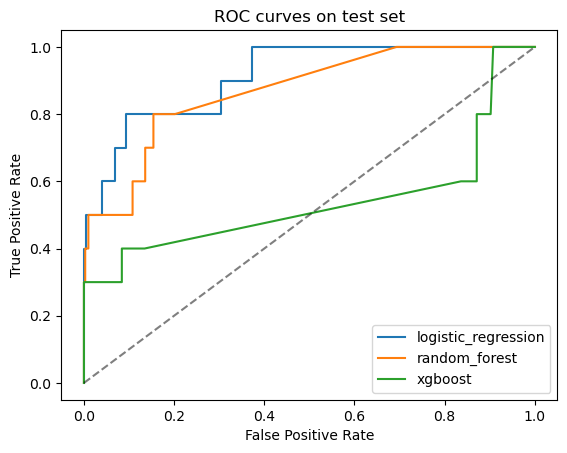
\includegraphics[width=0.75\textwidth]{roc_curves_test.png}
    \caption{ROC curves on the out-of-sample test set for all models.}
    \label{fig:roc_test}
\end{figure}

\begin{figure}[H]
    \centering
    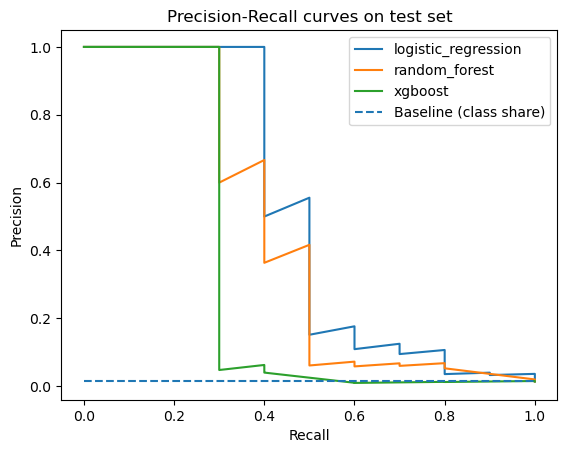
\includegraphics[width=0.75\textwidth]{pr_curves_test.png}
    \caption{Precision--Recall curves on the out-of-sample test set. The dashed line indicates the unconditional class frequency.}
    \label{fig:pr_test}
\end{figure}

\begin{figure}[H]
    \centering
    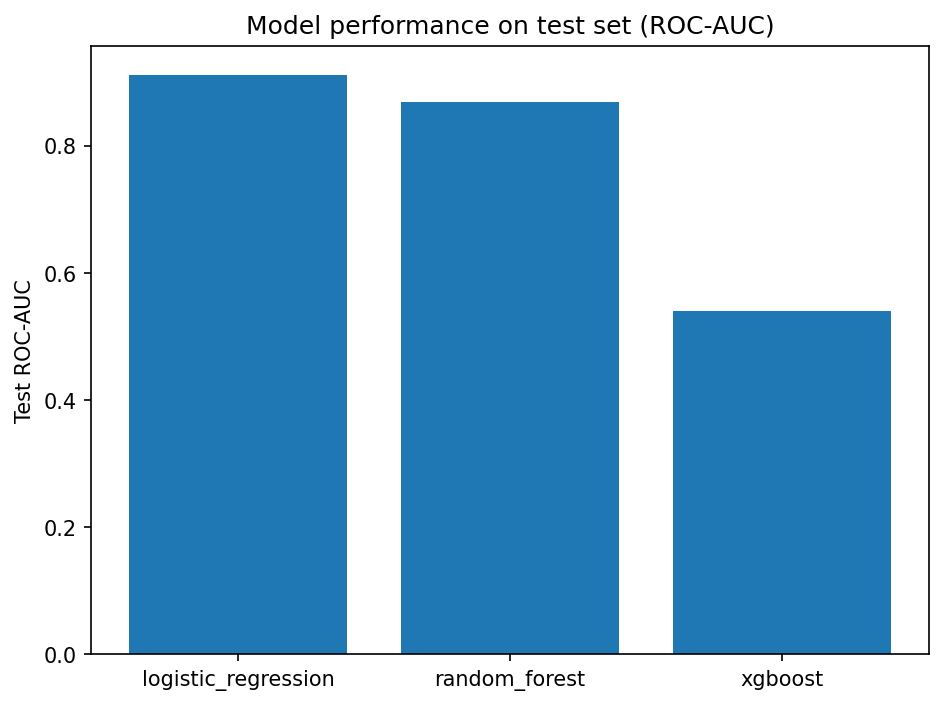
\includegraphics[width=0.75\textwidth]{test_roc_auc_barplot.png}
    \caption{Comparison of test ROC-AUC across models.}
    \label{fig:roc_bar}
\end{figure}

\begin{figure}[H]
    \centering
    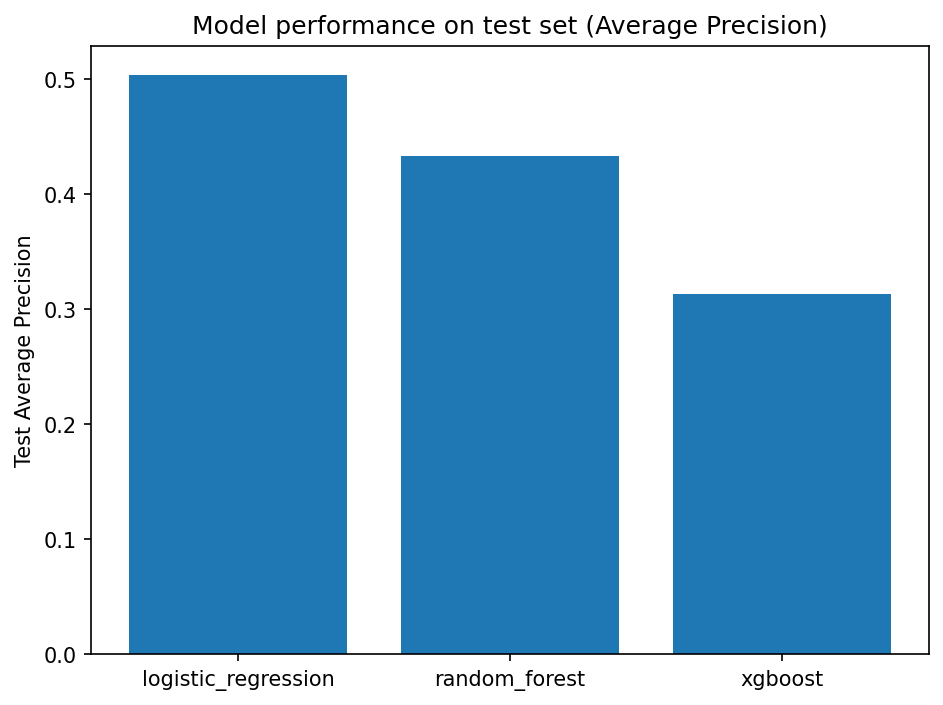
\includegraphics[width=0.75\textwidth]{test_avg_precision_barplot.png}
    \caption{Comparison of test Average Precision across models.}
    \label{fig:ap_bar}
\end{figure}

\begin{figure}[H]
    \centering
    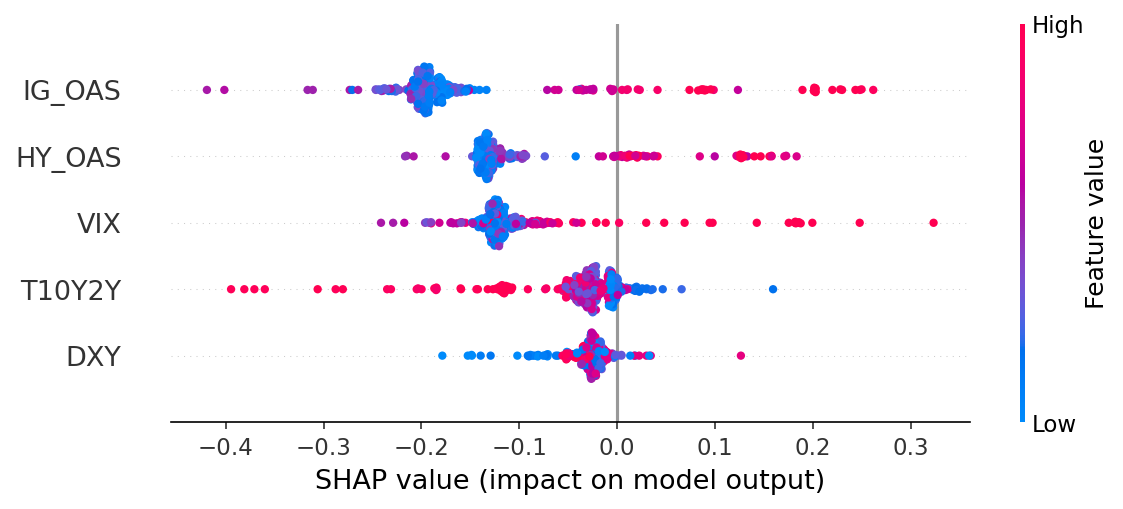
\includegraphics[width=0.80\textwidth]{shap_summary_random_forest.png}
    \caption{SHAP summary (beeswarm) plot for the Random Forest model.}
    \label{fig:shap_summary}
\end{figure}

\begin{figure}[H]
    \centering
    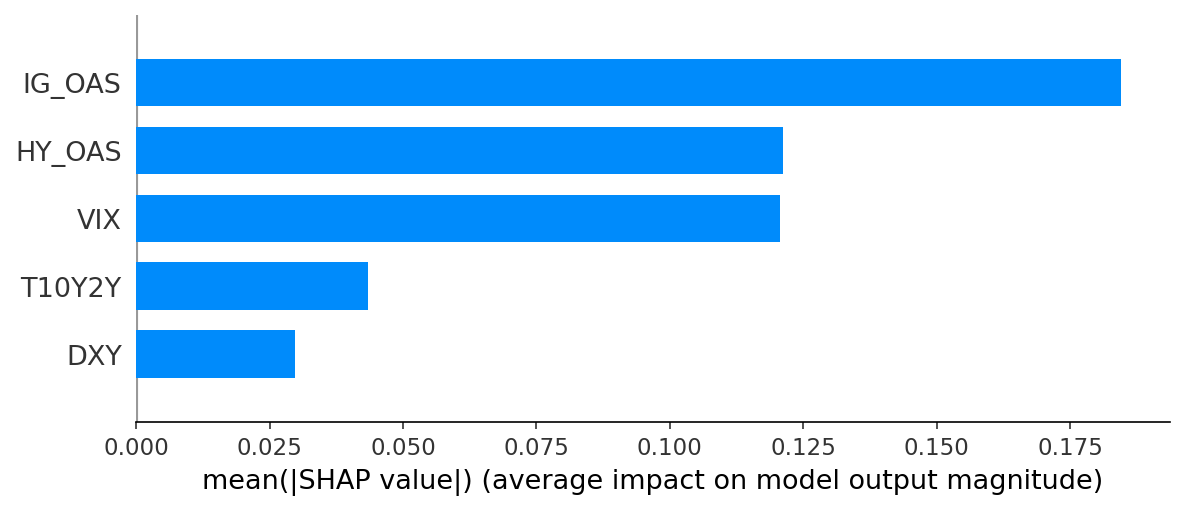
\includegraphics[width=0.80\textwidth]{shap_bar_random_forest.png}
    \caption{Mean absolute SHAP values for the Random Forest model.}
    \label{fig:shap_bar}
\end{figure}

\begin{figure}[H]
    \centering
    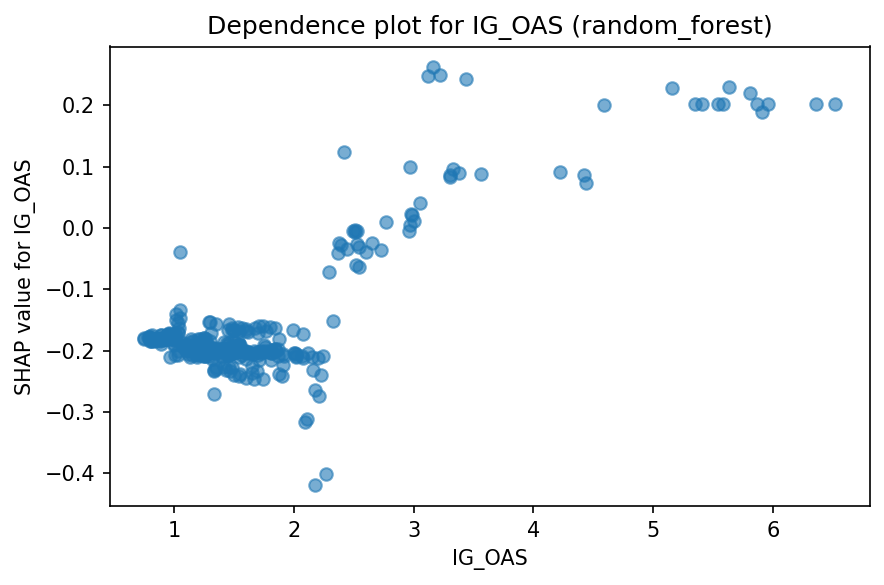
\includegraphics[width=0.80\textwidth]{shap_dependence_IG_OAS_random_forest.png}
    \caption{SHAP dependence plot for the IG\_OAS feature in the Random Forest model.}
    \label{fig:shap_dependence}
\end{figure}

\begin{figure}[H]
    \centering
    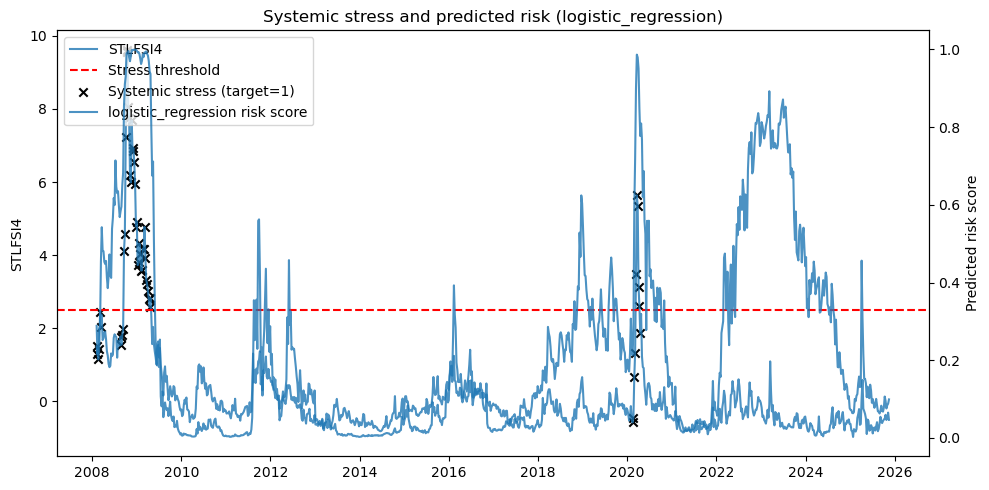
\includegraphics[width=0.95\textwidth]{timeline_logistic_regression.png}
    \caption{Temporal evolution of predicted risk scores from the Logistic Regression model alongside the STLFSI4 index.}
    \label{fig:timeline}
\end{figure}

\begin{figure}[H]
    \centering
    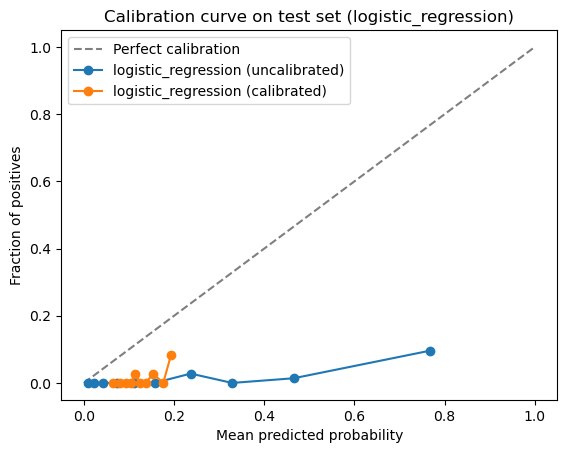
\includegraphics[width=0.85\textwidth]{calibration_curve_logistic_regression.png}
    \caption{Calibration curve for the Logistic Regression model on the test set, comparing uncalibrated and calibrated predicted probabilities.}
    \label{fig:calibration_logistic_regression}
\end{figure}

% ---------- Appendix C: AI Tools Usage ----------
\newpage
\section{AI Tools Usage}
\label{app:ai_usage}

Large language models (e.g.\ ChatGPT) were used as learning and support tools during the development of this project.

Specifically, AI assistance was used for:
\begin{itemize}
    \item debugging and interpretation of error messages,
    \item code review and refactoring suggestions,
    \item improving code readability, structure, and documentation,
    \item drafting and refining parts of the README and report text.
\end{itemize}

All modeling choices, data selection, feature engineering decisions, evaluation design, and interpretation of results were made independently by the author.

AI tools were not used to generate results, train models, select hyperparameters, manipulate data, or make automated modeling decisions.

The full codebase was reviewed, understood, and validated by the author. The final implementation, experimental results, and conclusions fully reflect the author’s own work.

% ================== References ==================
\newpage
\printbibliography

\end{document}